% #########################################################################
% #                       EXPLORACIÓN Y ANÁLISIS DE DATOS                 #
% #########################################################################

% Definición de nombres
\newcommand{\estudiante}{García Justel, Alan}
\newcommand{\titulo}{MÁSTER EN INGENIERÍA COMPUTACIONAL Y SISTEMAS INTELIGENTES}
\newcommand{\asignatura}{EXPLORACIÓN Y ANÁLISIS DE DATOS}
\newcommand{\portada}{common/no_signal.png}
\newcommand{\colorportada}{title_green}
\newcommand{\curso}{2024-2025}


% Notebook
\begin{document}
\newgeometry{bottom=2cm}

\begin{titlepage}
    % Logo de la universidad
    \begin{textblock*}{\textwidth}(2cm,0.4cm)
        \begin{center}
            \begin{minipage}{0.45\textwidth}
                \centering
                
\includegraphics[width=\textwidth]{common/Logo_EHU.jpg}
            \end{minipage}\hfill
            \begin{minipage}{0.45\textwidth}
                \centering
                
\includegraphics[width=0.8\textwidth]{common/Logo_KISA.png} 
            \end{minipage}
        \end{center}
    \end{textblock*}
    
    % Franja de color
    \begin{tikzpicture}[remember picture, overlay]
        \fill[\colorportada] (current page.north west) ++ (0,-3.01cm) rectangle (\paperwidth,-3cm);
    \end{tikzpicture}
    
    \begin{textblock*}{\paperwidth}(\dimexpr\parindent+\oddsidemargin+3em\relax,3.5cm)
        \begin{minipage}{\dimexpr\linewidth-7.5cm\relax}
            \color{white}
            \noindent\rule{\linewidth}{0cm}
            \textsf{ {\large \titulo}}
            \newline
            \newline \newline
            \textsf{\textbf{ {\Huge APUNTES DE ASIGNATURA }}}
        \end{minipage}
    \end{textblock*}
    
    % Nombre asignatura
    \vspace*{3.5cm}
    \begin{minipage}{\linewidth}
        \setlength{\baselineskip}{1.7\baselineskip}
        \centering
        \textsf{ \textbf{ {\LARGE \asignatura }}}
    \end{minipage}

    % Foto de portada
    \vspace*{0.5cm}
    \begin{figure}[H]
        \centering
        \includegraphics[width=10cm, height=8cm]{\portada}
    \end{figure}

    
    
    % Estudiante
    \vspace{0.2cm}
    \noindent {\footnotesize \textbf{Estudiante:} \estudiante}
    \newline
    \noindent\makebox[\linewidth]{\rule{\textwidth}{0.4pt}} % Línea horizontal

    % Curso y Fecha
    \vspace{0.1cm}    
    \noindent {\footnotesize \textbf{Curso: } \curso \hfill \textbf{Fecha:} \today }
\end{titlepage}

\restoregeometry
\setcounter{figure}{0} % Incluimos el título
\newpage
% Índices
\tableofcontents\thispagestyle{empty} \newpage
% \listoffigures\thispagestyle{empty}   %\newpage
% \listoftables\thispagestyle{empty}    %\newpage

\section{Introducción}
El análisis de datos es la actividad de transformar un conjunto de datos con le objetivo de extraer información útil y facilitar así la formulación de conclusiones. Inevitablemente, se va a trabajar con datos o conjuntos de objetos $\Omega = {w_1,\dots,w_n}$ de los que se van a extraer una serie de variables o características $X_1,\dots,X_p$, acotadas en un espacio de representación $X_j \rightarrow M_j, j = 1,\dots,p$ y que constituyen una aplicacion de forma que se consigue la descripción de los objetos en forma \textit{objeto - atributo - valor}:

\[
\begin{array}{c c c c}
    X_j: & \Omega & \rightarrow & M_j \\
         & w_i & \hookrightarrow & x_{ij}
\end{array}
\]

Durante este curso se utilizará la notación $n \times p$: individuos por filas y atributos por columnas. Sin embargo, a la hora de referirse a un único individuo siempre se hará en forma de vector columna (cada fila es un atributo).
\ex{Notación}{
    \[
        \begin{blockarray}{cccc}
            & X_1 & X_2 & X_3 \\
            \begin{block}{c[ccc]}
                w_1 & 0.76 & 5    & 1.3 \\
                w_2 & 1.20 & 0    & 1.2 \\
                w_3 & 0.70 & 4    & 1.3 \\
                w_4 & 0.12 & 7    & 1.6 \\
                w_5 & 0.94 & 3    & 1.9 \\
            \end{block}
        \end{blockarray}_{5 \times 3}
    \]
}

Existen numerosas técnicas en el análisis de datos y es difícil hacer una clasificación exahustiva. A pesar de ello, sí que se pueden diferenciar dos grandes bloques:
\begin{itemize}
    \item \textbf{Técnicas no supervisadas:} reducción de dimensión (ACP, MDS, \dots); clustering (k-means, jerárquico, mixturas \dots)
    \item \textbf{Técnicas supervisadas:} clasificación (Discriminante Lineal, k-NN, Árboles de clasificación, redes neuronales, SVM, reg. logística, \dots),
    regresión (lineal, no-paramétrico, GAM, Ridge, redes neuronales, SVM, \dots)
\end{itemize}

En cuanto a los datos, existen dos tipos:
\begin{itemize}
    \item \textbf{Variables Cualitativas:} 
\end{itemize} 

\subsection{Estadísticos principales}
Un estadístico es un número que resume cierta característica de los datos como la tendencia central o la dispersión.

\subsubsection{Variables Cuantitativas}
Las variables cuantitativas son aquellas en las que los valores de las variables se pueden cuantificar numéricamente. Existen dos tipos:

\begin{itemize}
    \item \textbf{Discretas:} el rango de la variable es finito o numerable.
    \item \textbf{Contínuas:} el rango de la variable contiene un intervalo de la Recta Real.
\end{itemize}

Para cualquiera de los dos tipos se presentan las siguientes definiciones de los estadísticos principales para variables cuantitativas:

\dfn{Meida aritmética}{
    \begin{gather*}
        \mean{x}_j = \frac{1}{n} \sum_{i=1}^{n}x_{ij} \text{ donde } j = 1,\dots,p \\
        \mean{x}^t = \frac{1}{n} \textbf{1}^tX \text{ donde } \textbf{1}=(1,\dots,n)^t
    \end{gather*}
}
\dfn{Varianza y desviación típica}{
    \begin{gather*}
        s^2_j = \frac{1}{n - 1} \sum_{i=1}^{n}(x_{ij} - \mean{x}_j)^2 \\
        s_j = \sqrt{s^2_j} \text{ donde } j = 1,\dots,p
    \end{gather*}
}
\dfn{Covarianza entre $X_i$ y $X_j$}{
    \begin{gather*}
        s_{ij} = \frac{1}{n-1} \sum_{l=1}^{n}(x_{li} - \mean{x}_i)(x_{lj} - \mean{x}_j) \\ = \frac{1}{1-n}SX_iX_j \text{ donde }
        S = \begin{pmatrix}
            s^2_{11} & s_{12} & \dots & s_{1p} \\
            s_{21} & s^2_{22} & \dots & s_{2p} \\
            \vdots & \vdots & \ddots & \vdots \\
            s_{p1} & s_{p2} & \dots & s^2_{pp}
        \end{pmatrix}
    \end{gather*}
}
Con una matriz de correlaciones solo podemos capturar o identificar relaciones lineales. La matriz de varianzas-covarianzas $S$ es una matriz simétrica que depende de las unidades de medición, por lo que para buscar relaciones lineales entre variables es necesario normalizar los estadísticos. Es aquí donde entra el coeficiente de correlación de Pearson.
\dfn{Correlación}{
    \[
        r_{ij} = \frac{s_{ij}}{s_is_j} \text{ o forma matricial }
        R = \begin{pmatrix}
            1      & r_{12} & \dots & r_{1p} \\
            r_{21} & 1      & \dots & r_{2p} \\
            \vdots & \vdots & \ddots & \vdots \\
            r_{p1} & r_{p2} & \dots & 1
        \end{pmatrix}
    \]

    Sea $r_{ij}$ la correlación entre las variables $X_i$ y $X_j$. Entonces,
    \[
    -1 \leq r_{ij} \leq 1 \text{ } i,j = 1,\dots,p\text{.} 
    \]
    \begin{itemize}
        \item $r_{ij} = 0$, no hay asociación \textbf{lineal} entre  $X_i$ y $X_j$
        \item $r_{ij} > 0$, asociación \textbf{lineal} positiva entre  $X_i$ y $X_j$
        \item $r_{ij} < 0$, asociación \textbf{lineal} negativa entre  $X_i$ y $X_j$
    \end{itemize}
}

\subsubsection{Variables Cualitativas}
Las variables cualitativas son aquellas en las que los valores de las variables representan cualidades. Podemos distinguir dos tipos principales:

\begin{itemize}
    \item \textbf{Binarias:} aquellas en las que solo hay dos valores posibles
    \item \textbf{Nominales:} aquellas en las que hay más de dos valores posibles
\end{itemize}

En cualquiera de los casos, al tratar con variables cualitativas es necesario generar una tabla de frecuencias, con lo que una tabla de contingencia es muy útil para identificar relaciones entre los datos:

\[
\begin{array}{c|ccccc|c}
    X \setminus Y & y_1 & \cdots & y_j & \cdots & y_m& \text{Totales} \\
    \hline
    x_1 & n_{11} & \cdots & n_{1j} & \cdots     & n_{1m} & n_{1\bullet}  \\
    \vdots & \vdots & \ddots & \vdots & \ddots  & \vdots & \vdots     \\
    x_i & n_{i1} & \cdots & n_{ij} & \cdots     & n_{im}& n_{i\bullet}  \\
    \vdots & \vdots & \ddots & \vdots & \ddots  & \vdots & \vdots     \\
    x_l & n_{l1} & \cdots & n_{lj} & \cdots     & n_{lm}& n_{l\bullet}  \\
    \hline
    \text{Totales} & n_{\bullet 1} & \cdots & n_{\bullet j} & \cdots & n_{\bullet m} & n
\end{array}
\]

Algunos estadísticos para medir la asociación entre datos de variables cualitativas son los siguientes:

\dfn{Chi-cuadrado}{
    \[
        \chi^2 = \sum_{i=1}^{l} \sum_{j=1}^{m} \frac{(n_{ij} - n_{i\bullet}n_{\bullet j} / n)^2}{n_{i\bullet}n_{\bullet j} / n}
    \]

    Sea $r_{ij}$ la correlación entre las variables $X_i$ y $X_j$. Entonces,
    \[
    -1 \leq r_{ij} \leq 1 \text{ } i,j = 1,\dots,p\text{.} 
    \]
    \begin{itemize}
        \item $r_{ij} = 0$, no hay asociación.
        \item $r_{ij} > 0$, cuanto mayor sea $\chi^2$ mayor es la asociación.
    \end{itemize}
}
\dfn{Coeficiente de contingencia}{
    \begin{gather*}
        C = (\frac{\chi^2}{\chi^2 + n})^{\frac{1}{2}}\\
        0 \leq C \leq 1
    \end{gather*}
    $C = 0 $, ausencia de asociación.
}

\dfn{Información mútua}{
    \[
        I = \sum_{i=1}^{l} \sum_{j=1}^{m} \frac{n_{ij}}{n}\log \frac{n_{ij}}{n_{i\bullet}n_{\bullet j} / n}
    \]
    \begin{itemize}
        \item $I = 0$, no hay asociación.
        \item Cuanto mayor sea $I$ mayor es la asociación.
    \end{itemize}
}


\ex{Media en variables binarias}{
    \[
        X = \text{'Tiene una anomalía'}
    \]
    \[
        X = 
        \begin{pmatrix}
            0 \\
            1 \\
            0 \\
            0 \\
            0
        \end{pmatrix}
        \quad \mean{X} = \frac{1}{5} = 0.2
    \]
    Nos devuelve la frecuencia del 1 (probabilidad de que ocurra 1)
}



\subsection{Exploración Gráfica con R}
Existen dos librerías base para graficar con R. Por un lado contamos con las funciones básicas provistas por la librería estándar de R con las que podemos realizar exploraciones rápidas y sencillas y por otro lado contamos con la librería \textit{ggplot2} para realizar gráficas más avanzadas.

En R base hay varias paletas de colores: colors, rainbow. . . pero además, hay diversos paquetes para manejar colores, por ejemplo RColorBrewer, que permiten marcar contrastes, o graduaciones en la escala de colores.

\nt{}{
    \begin{itemize}
        \item \textbf{plot::pch} $\rightarrow$ Valor para los plots que indican el icono del punto a plotear (0: 25)
    \end{itemize}
}

\qs{Obtén una serie de gráficos a partir de estos datos}{
    {\tiny
    
    Entre los estudios que realiza periódicamente EUSTAT está el del uso del tiempo que hacemos. En este apartado trabajaremos con datos (TiempoActividad.csv) derivados de este tiempo. Las variables que tenemos son:
    \begin{itemize}
        \item SEXO
        \item EDAD (categorizada)
        \item HORARIO (0: Sin ocupación; 1: Jornada sin trabajo; 2: Trabajo sin horario; 3: Horario de mañana o normal; 4: Horario de tarde; 5: Horario de noche)
        \item JORNADA (SinOcup: Sin ocupación; Normal: Día de trabajo normal; MediaJ: Día de media jornada laboral; DescansoNOTRAB: Día de descanso festivo no trabajado; DescansoSITRAB: Día de descanso o festivo trabajado; BajaEnf : Día de baja por enfermedad; Festivo: Día de vacaciones; Otros: Otros casos)
        \item TiempoLAB (Duración de la actividad a un dígito <<Trabajo profesional y tiempo de formación>> (segundos))
        \item TiempoCUIDADO (Duración de la actividad a un dígito <<Cuidados a las personas del hogar>> (segundos))
        \item DIASEMANA (1: Lunes; — 7: Domingo)
    \end{itemize}
    }
}

\sol 
\begin{figure}[H]
    \centering
    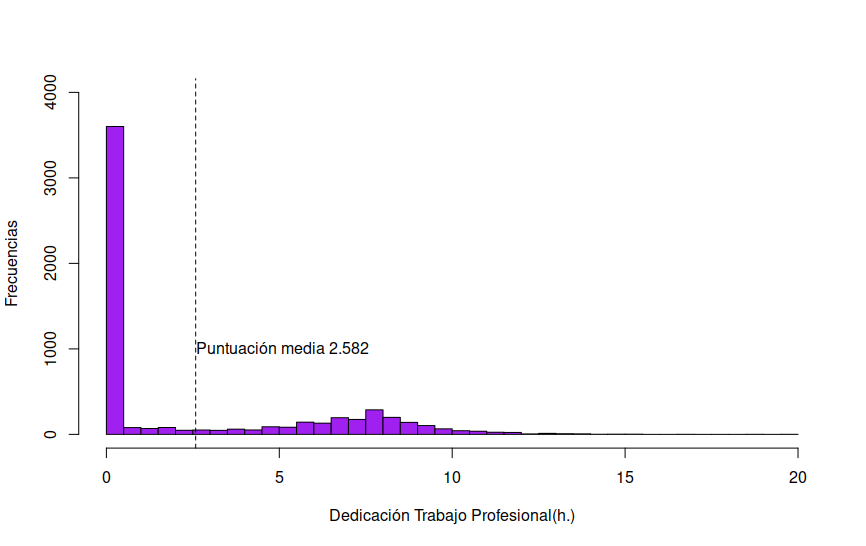
\includegraphics[width=0.6\linewidth]{EAD/images/Ejercicio_T1_E01_01.png}
    \vspace{0.5cm}
    \begin{minipage}{0.49\textwidth}
        \centering
        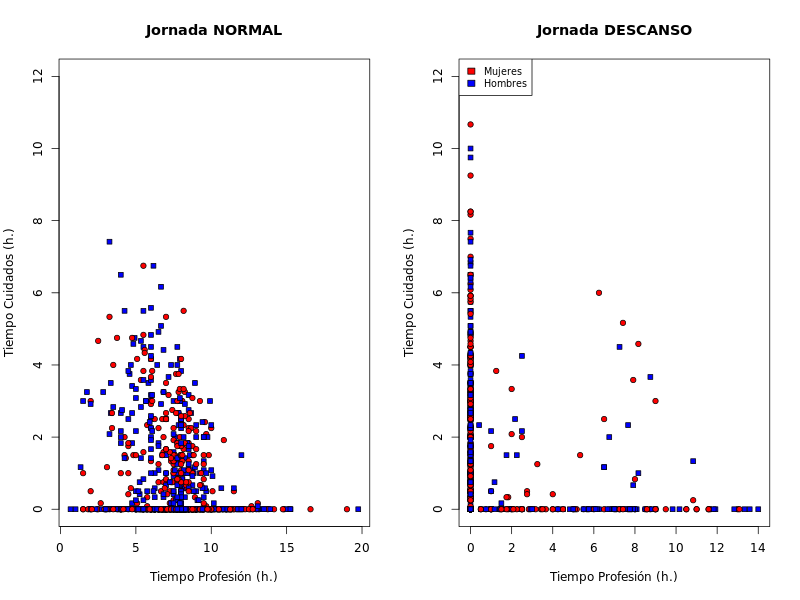
\includegraphics[width=0.7\linewidth]{EAD/images/Ejercicio_T1_E01_02.png}
    \end{minipage}
    \hfill
    \begin{minipage}{0.49\textwidth}
        \centering
        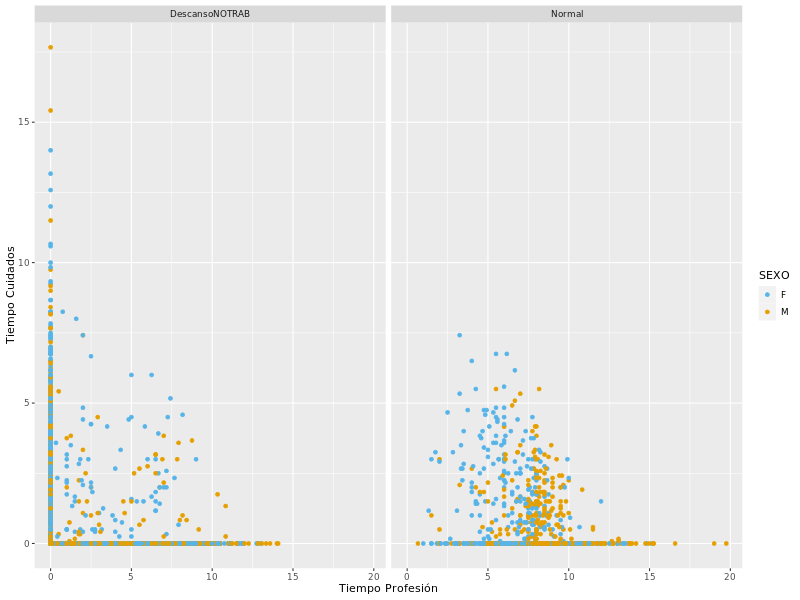
\includegraphics[width=0.7\linewidth]{EAD/images/Ejercicio_T1_E01_03.png}
    \end{minipage}
    
    \caption{Gráficas resultado del ejercicio. El código se puede encontrar en la carpeta de ejercicios}
\end{figure}



\section{Tema 2}
\subsection{Repaso Álgebra}
El producto escalar es la sombra de un vector sobre otro
Si centramos dos veces tenemos la matriz de varianzas covarianzas
Vectores propios y valores propios

\subsection{Distancias, similaridades y kernels}
Una distancia o similaridad se define como

Además, se dice que una distancia es una métrica si se cumple

En otras palabras que la distancia de un sitio a otro es la más corta (como en el plano es la recta)

La matriz de similaridad se diferencia de la de la distancia en que la similaridad de uno consigo mismo es uno en lugar de 0 (como ocurre con la distancia)

Tipos de distancias para variables cuantitativas:
- Distancia euclídea
- Distancias de Minkowsky (generalización de la distancia euclídea)
- Distancia de Karl Pearson. Tengo dos personas que miden(m) y pesan(kg): w_1(1.65, 70) y w_2(1.75, 72) -> distancia euclidea -> 0.1² + 2². El problema es que la altura queda muy diluida respecto al peso. Por ello hay que hacer una estandarización. Es similar a la distancia de Mahalanobis solo que solo se utiliza la matriz diagonal de varianzas.
- Distancia de Mahalanobis. Puede dar problemas si en un mismo conjunto de datos existen  distintas distribuciones o agrupaciones inconsistentes (una regresión y una agrupación por ejemplo).


En el caso de variables binarias, lo más común es calcular similaridades en lugar de distancias (calcular las coincidencias en una tabla de contingencia).

Tipos de similaridades:
- Similaridad de (simétrica)
- Similaridad de Jaccard (asimétrica)

\ex{Similaridad binaria simétrica / asimétrica}{
X_1 = 'Animal Adulto (1) / Cría (0)'
X_2 = 'Tiene 4 patas (sí, no)'

gallina -> (0, 0)
serpiente -> (0, 0)
De esta manera, la gallina y la serpiente se parece. Sin embargo, es más pertinente preguntarse si la pregunta de ¿Tiene 4 patas? es adecuada.
el 0, 0 para las 4 patas no lo quiero contar, las no coincidencias no me interesan luego X_2 debe tratarse de forma asimétrica. Pero por otro lado X_1 sí que me aporta información relevante en las coincidencias de (0, 0) (ambos animales son crías y por lo tanto se parecen), luego es adecuado tratarla de forma simétrica.
}

\ex{¿Similaridades / distancias entre los objetos?}{
Similaridad simétrica
\[
S_{3x3} = \begin{bmatrix}
    1 & 4/6 & 1/6 \\
    0 & 1 & 3/6 \\
    0 & 0 & 1
\end{bmatrix}
\]
Similaridad asimétrica
}
\nt{dist(method = "binary") en R}{
    Esta distancia devuelve d_{ij} = 1 - S_{ij} donde S es el índice Jaccard.
}

\subsection{Distancias, similaridades y kernels}
\subsection{Reducción dimensionalidad}
\subsection{Clustering}

\end{document}